\vspace{-21mm}
\section{Artificial Boundaries at the Surface and Far--Field}
\label{intro:analysis_near_surface_and_far_field}

We then asked the natural question -- what happens if the artificial boundaries imposed at $\{z=a\}$ and $\{z=b\}$ are close to the interfacial surface $z=g(x)$? Can our HOPS/AWE algorithm converge if the artificial boundaries are moved below the grating surface? To investigate, we set $\Eps = 10^{-8}$ and changed the artificial boundaries to 
\vspace{-1mm}
\bes
a=10^{-6},\quad b=-10^{-6}, 
\ees
where the physical parameters were $(5.22)$ and numerical discretization was $(5.23)$ so that the artificial boundaries are above the grating surface. In Figure $17$, we simultaneously increased $N$ and $M$ to $N=M=4$ and $N=M=16$ Taylor orders as $\varepsilon$ decreased.
\vspace{-24.5mm}
\begin{figure}[H]
    \subfloat[\centering $N=M=4, \varepsilon=10^{-8}$ ]
    {{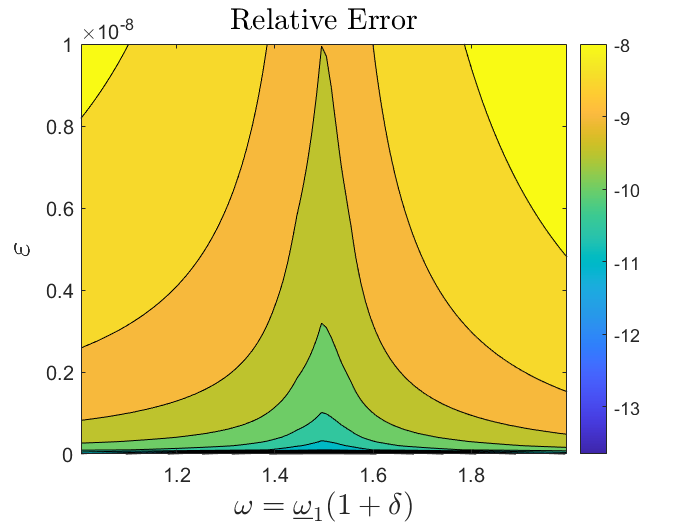
\includegraphics[width=7.6cm]{sections/5_method_of_maufactured_solutions/MMS_N_M_4_Upper_Field_Eps_1e-8_AB_1e-6.png} }}
    \subfloat[\centering $N=M=16, \varepsilon=10^{-8}$ ]
    {{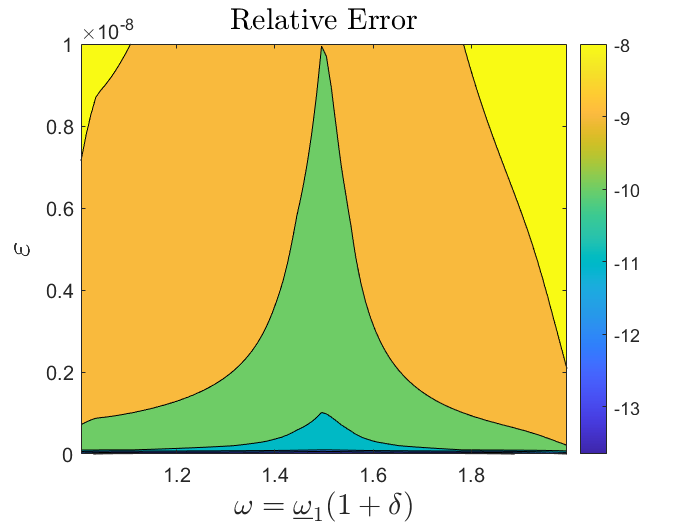
\includegraphics[width=7.6cm]{sections/5_method_of_maufactured_solutions/MMS_N_M_16_Upper_Field_Eps_1e-8_AB_1e-6.png} }}
%\includegraphics[width=0.5\textwidth]{conv_Eps}
\vspace{1mm}
\caption{Plot of relative error in the upper layer with the artificial boundaries imposed at $a=10^{-6}$ and $b=-10^{-6}$. Physical parameters were $(5.22)$ and numerical discretization was $(5.23)$.}
\label{Fig:Eps}
\end{figure}
\vspace{-14mm}
With these, we see that our HOPS/AWE algorithm returns satisfactory results with $N=M=4$ Taylor orders. At $N=M=16$ Taylor orders we obtain good results comparable to that of Figure $14$ where the artificial boundaries are imposed at $\{a=1\}$ and $\{b=-1\}$. We speculate that our HOPS/AWE algorithm will always converge provided we have a good profile and impose artificial boundaries above the surface. To validate this hypothesis, we set $\Eps = 10^{-8}$ and changed the artificial boundaries to
\bes
a=10^{-12},\quad b=-10^{-12},   
\ees
which are below the grating surface. In Figure $18$, we calculate $N=M=4$ and $N=M=16$ Taylor orders as $\varepsilon$ decreases.
\vspace{-17mm}
\begin{figure}[H]
    \subfloat[\centering $N=M=4, \varepsilon=10^{-8}$ ]
    {{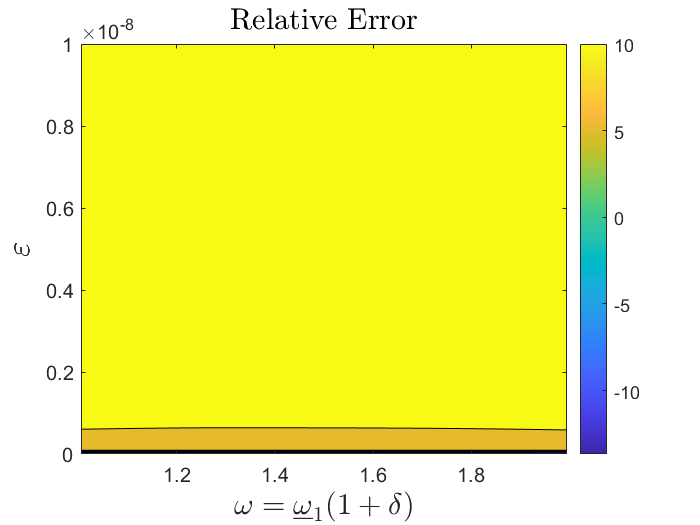
\includegraphics[width=7.6cm]{sections/5_method_of_maufactured_solutions/MMS_N_M_4_Upper_Field_Eps_1e-8_AB_1e-12.png} }}
    \subfloat[\centering $N=M=16, \varepsilon=10^{-8}$ ]
    {{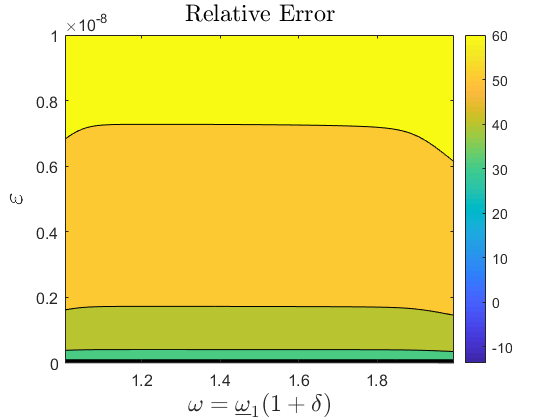
\includegraphics[width=7.6cm]{sections/5_method_of_maufactured_solutions/MMS_N_M_16_Upper_Field_Eps_1e-8_AB_1e-12.png} }}
%\includegraphics[width=0.5\textwidth]{conv_Eps}
\vspace{3mm}
\caption{Plot of relative error in the upper layer with the artificial boundaries imposed at $a=10^{-12}$ and $b=-10^{-12}$. Physical parameters were $(5.22)$ and numerical discretization was $(5.23)$.}
\label{Fig:Eps}
\end{figure}
\vspace{-18mm} The results of Figure $18$ show that higher Taylor orders do not compensate for moving the computational domain below the grating surface. Therefore, irregardless of how many Taylor orders we compute, we still see disastrous results with our HOPS/AWE algorithm. The domain--flattening change of variables introduced in $\S 2.4$ is only applicable to a domain decomposition where the artificial boundaries are above the surface in the upper layer and below the surface in the lower layer. Further testing against comparable profiles demonstrates that our HOPS/AWE algorithm meets a threshold whenever the artificial boundary is smaller than the perturbation parameter $\varepsilon$ and is below the surface of the interface.
\newline
\\
Next, we investigated imposing artificial boundaries at values of $\{z=a\}$ and $\{z=b\}$ that are far away from the interfacial surface. As with the boundaries near the grating surface, we suspect that the accuracy of our HOPS/AWE algorithm will be constrained by the amount of Taylor orders necessary to recover far--field data through our elliptic solver. For our test profile we once again selected the physical parameters in $(5.22)$ and numerical discretization in $(5.23)$ where we increased the artificial boundaries to
\bes
a=10^{6},\quad b=-10^{6},
\ees
and then 
\bes
a=10^{12},\quad b=-10^{12},
\ees
and
\bes
a=10^{18},\quad b=-10^{18}.
\ees
These three choices allow us to simulate a larger computational domain where our elliptic solver will recover far--field data from an interfacial data structure. We also extended the number of collocation points in $(5.23)$ to
\bes
N_z=1000 \quad \text{and} \quad N_z = 10,000,
\ees
where we observed no difference between simulating $N_z=32$, $N_z=1000$, or $N_z=10,000$ collocation points. In Figure $19$ we report the results of setting $\Eps = 10^{-2}$ with $N=M=4$ Taylor orders and $\Eps = 10^{-8}$ with $N=M=16$ Taylor orders where we impose the artificial boundaries of $\{a=10^{6}\}$ and $\{b=-10^{6}\}$. Then in Figures $20$ and $21$ we simulate the same values of $\Eps$ and the same Taylor orders against the artificial boundaries of $\{a=10^{12}\}, \{b=-10^{12}\}$ and $\{a=10^{18}\}, \{b=-10^{18}\}$.
\vspace{-14mm}
\begin{figure}[H]
    \subfloat[\centering $N=M=4, \varepsilon=10^{-2}$ ]
    {{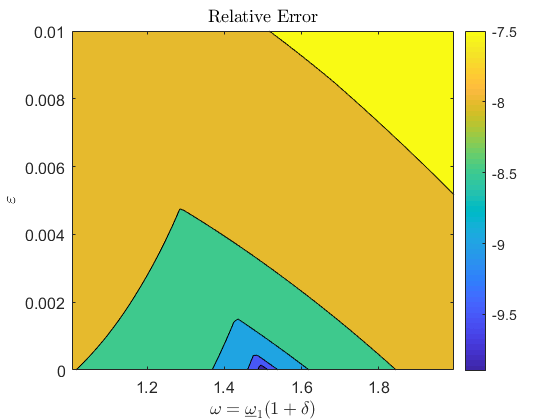
\includegraphics[width=7.6cm]{sections/5_method_of_maufactured_solutions/MMS_N_M_4_Upper_Field_Eps_1e-2_AB_1e+6.png} }}
    \subfloat[\centering $N=M=16, \varepsilon=10^{-8}$ ]
    {{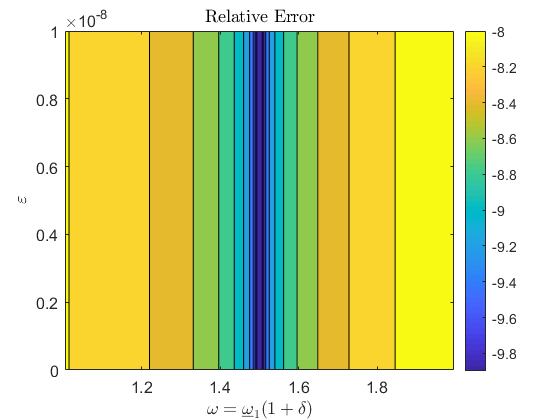
\includegraphics[width=7.6cm]{sections/5_method_of_maufactured_solutions/MMS_N_M_16_Upper_Field_Eps_1e-8_AB_1e+6.png} }}
%\includegraphics[width=0.5\textwidth]{conv_Eps}
\vspace{3mm}
\caption{Plot of relative error in the upper layer with the artificial boundaries imposed at at $a=10^{6}$ and $b=-10^{6}$. Physical parameters were $(5.22)$ and numerical discretization was $(5.23)$.}
\label{Fig:Eps}
\end{figure}

\begin{figure}[H]
    \subfloat[\centering $N=M=4, \varepsilon=10^{-2}$ ]
    {{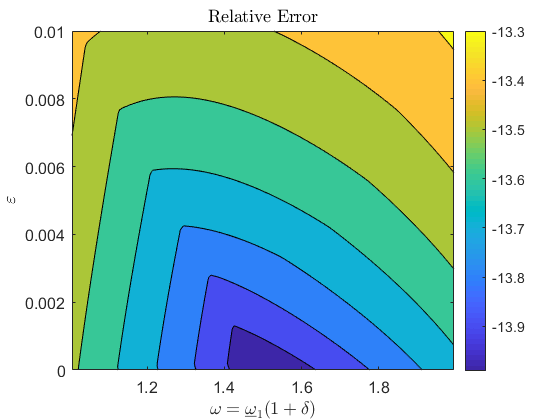
\includegraphics[width=7.6cm]{sections/5_method_of_maufactured_solutions/MMS_N_M_4_Upper_Field_Eps_1e-2_AB_1e+12.png} }}
    \subfloat[\centering $N=M=16, \varepsilon=10^{-8}$ ]
    {{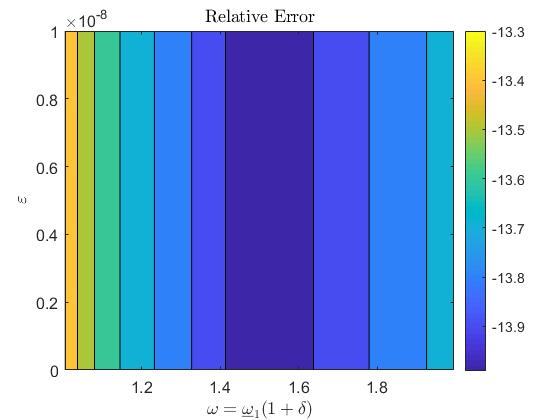
\includegraphics[width=7.6cm]{sections/5_method_of_maufactured_solutions/MMS_N_M_16_Upper_Field_Eps_1e-8_AB_1e+12.png} }}
%\includegraphics[width=0.5\textwidth]{conv_Eps}
\vspace{3mm}
\caption{Plot of relative error in the upper layer with the artificial boundaries imposed at at $a=10^{12}$ and $b=-10^{12}$. Physical parameters were $(5.22)$ and numerical discretization was $(5.23)$.}
\label{Fig:Eps}
\end{figure}

\vspace{-39mm}
\begin{figure}[H]
    \subfloat[\centering $N=M=4, \varepsilon=10^{-2}$ ]
    {{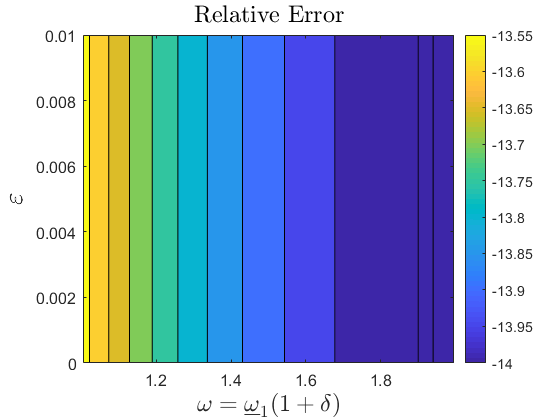
\includegraphics[width=7.6cm]{sections/5_method_of_maufactured_solutions/MMS_N_M_4_Upper_Field_Eps_1e-2_AB_1e+18.png} }}
    \subfloat[\centering $N=M=16, \varepsilon=10^{-8}$ ]
    {{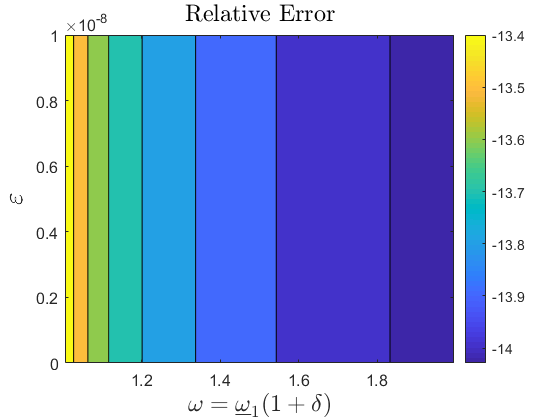
\includegraphics[width=7.6cm]{sections/5_method_of_maufactured_solutions/MMS_N_M_16_Upper_Field_Eps_1e-8_AB_1e+18.png} }}
%\includegraphics[width=0.5\textwidth]{conv_Eps}
\vspace{3mm}
\caption{Plot of relative error in the upper layer with the artificial boundaries imposed at at $a=10^{18}$ and $b=-10^{18}$. Physical parameters were $(5.22)$ and numerical discretization was $(5.23)$.}
\label{Fig:Eps}
\end{figure}
\vspace{-16mm}
The results of Figures $19,20,$ and $21$ are counterintuitive. As we move the artificial boundaries further away from the surface of the interface, we would expect that our HOPS/AWE algorithm would perform poorly due to the extra amount of computation necessary to resolve the elliptic solver in the far--field. However, further testing validates that our HOPS/AWE algorithm is better suited towards a larger computational domain. It is unclear why increasing the height of the computational domain improves the accuracy of the DNO solver in our HOPS/AWE algorithm.